\section{Ejercicio 5}

$$
F(A,B,C,D) = \prod(0,1,4,6,7,8,9,13,15)
$$

\subsection{Expresión mínima}

\begin{figure}[H]
    \centering
    \begin{karnaugh-map}[4][4][1][$D$][$C$][$B$][$A$]
        \maxterms{0,1,4,6,7,8,9,13,15}
        \minterms{2,3,5,10,11,12,14}
        \implicant{5}{5}
        \implicantedge{12}{12}{14}{14}
        \implicantedge{3}{2}{11}{10}
    \end{karnaugh-map}
    \caption{Mapa de Karnaugh para la función}
\end{figure}

$$
F(A,B,C,D) = \overline{B}C + \overline{A}B\overline{C}D + AB\overline{D}
$$

\subsection{Simulación en Falstad}
\begin{figure}[H]
    \centering
    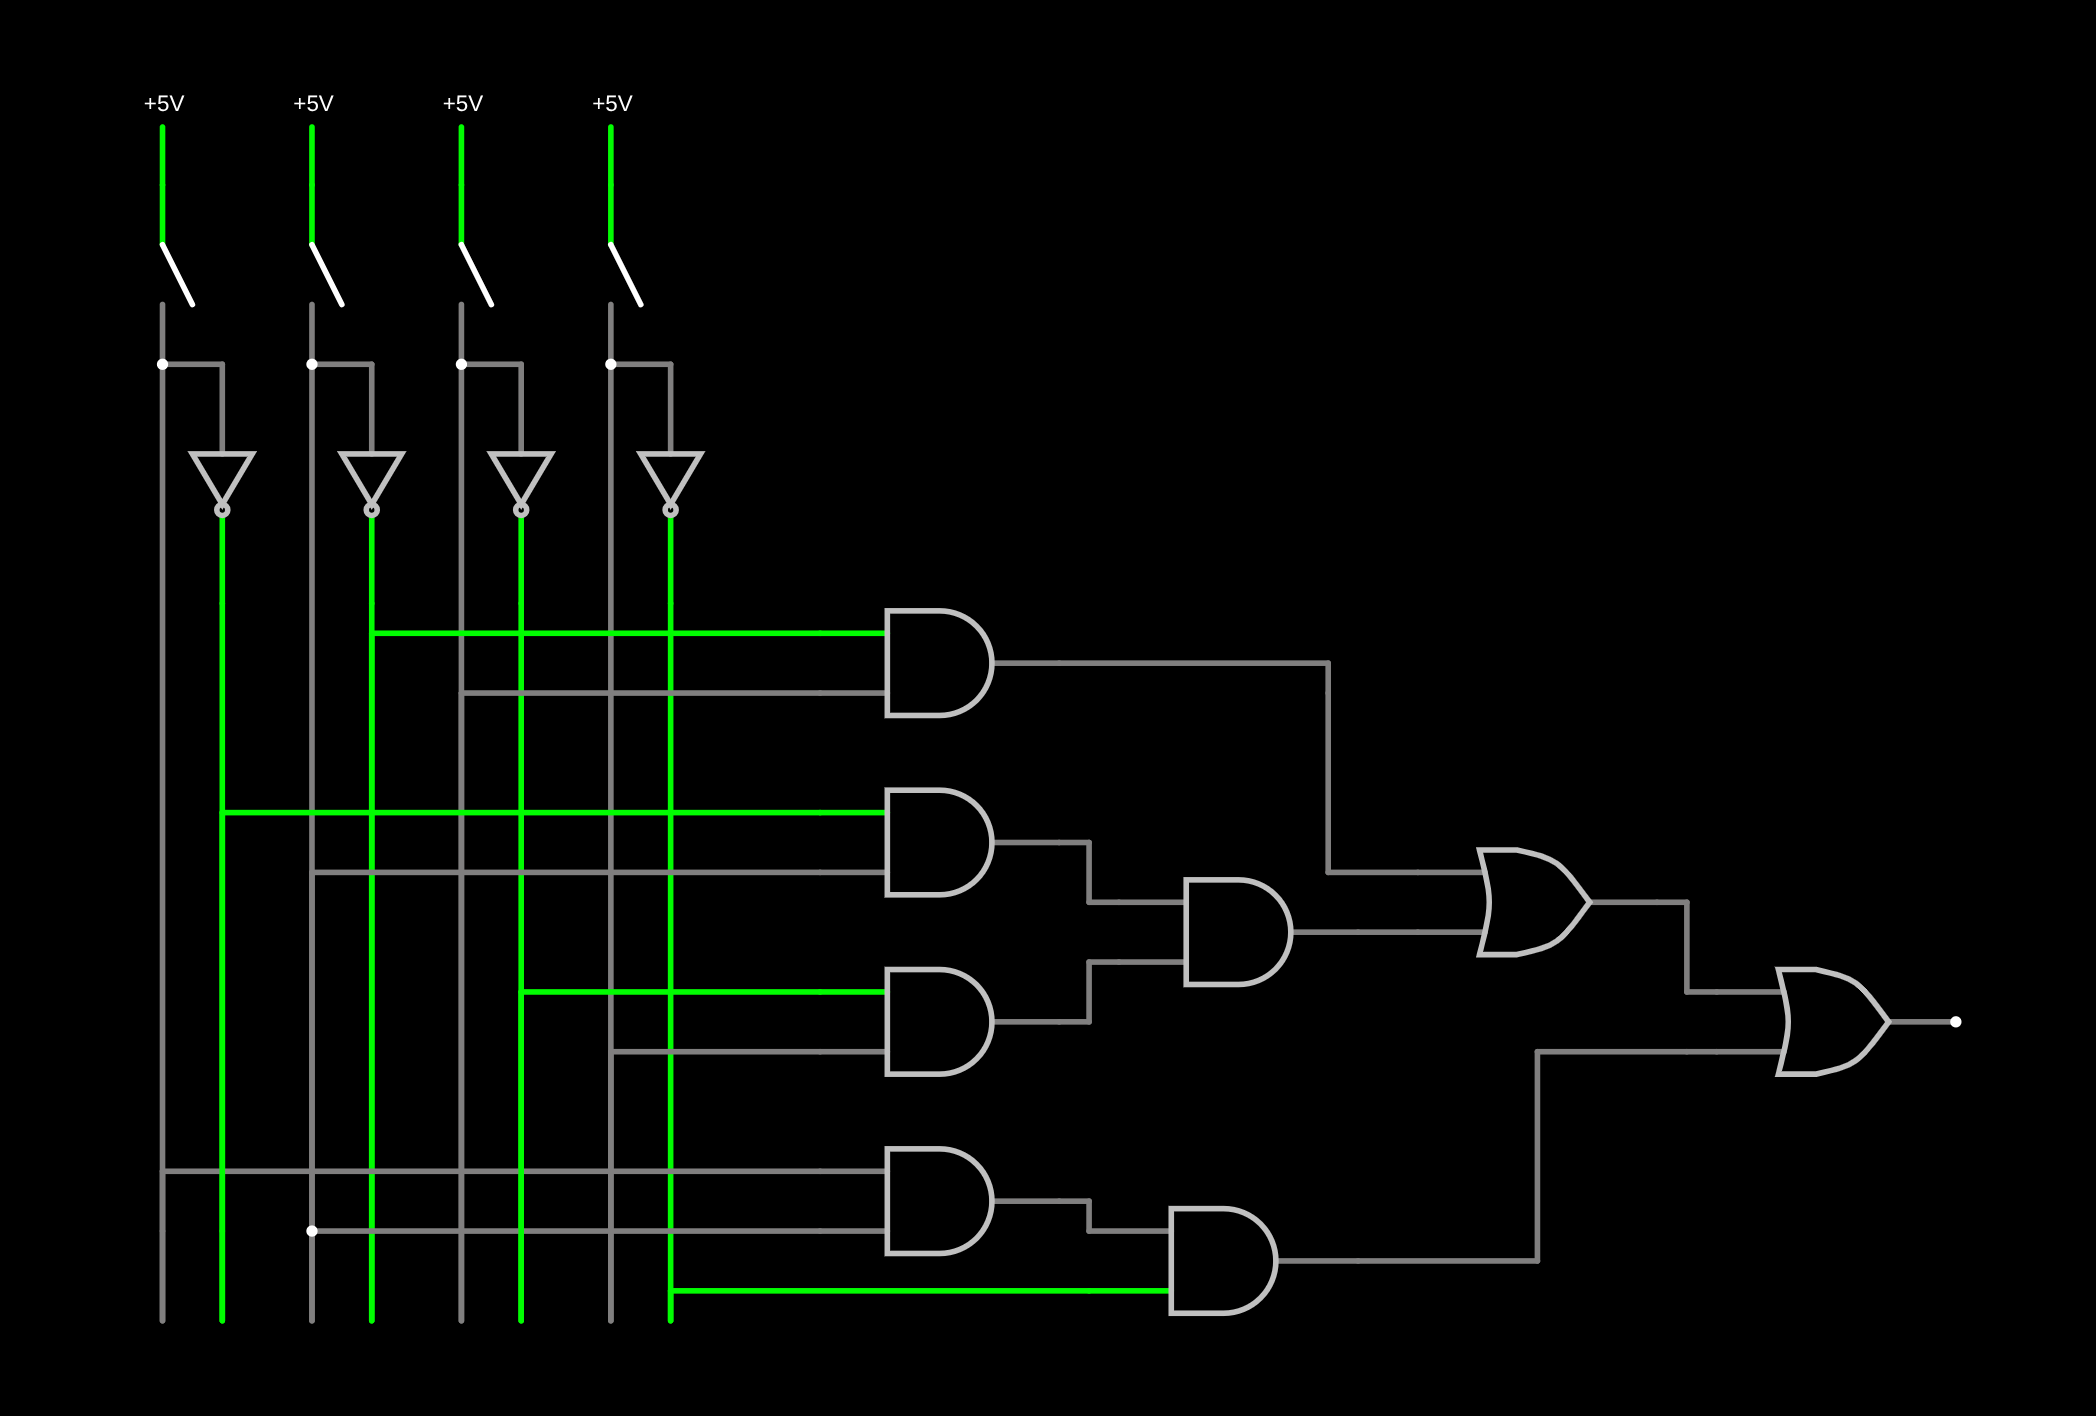
\includegraphics[width=0.6\textwidth]{img/Falstad/ej8.png}
    \caption{Simulación de la función en Falstad}
\end{figure}

\subsection{Descripción en Verilog}

\begin{Verbatim}[ frame=single, fontsize=\small, baselinestretch=1.2 ]
module ej8 (
    input A,
    input B,
    input C,
    input D,
    output F
);

assign F = ~B&C | ~A&B&~C&D | A&B&~D;

endmodule
\end{Verbatim}

\subsection{Captura del RTL}
\begin{figure}[H]
    \centering
    
\includegraphics[width=0.8\textwidth]{img/Xilinx/ej8.png}
    \caption{Captura del RTL en Xilinx}
\end{figure}